\documentclass[main.tex]{subfiles}
\begin{document}

\chapter{Characteristic Functions and the Central Limit Theorem}\label{ch:clt}\chaptermark{Characteristic Functions and the CLT}

The Law of Large Numbers says that $\bar X_n$ converges to $\mu$, but it does not say \emph{how}, i.e.\ what the distribution of the error $\bar X_n-\mu$ looks like. The Central Limit Theorem (CLT\index{central limit theorem clt@central limit theorem (CLT)}) states that this error, scaled by $\sqrt n$, converges to a normal distribution --- whatever the initial distribution. Almost all approximate confidence intervals, $z$- and Wald tests\index{wald test@Wald test} and the asymptotic theory of the MLE are consequences of this theorem. The main tool of the proof is the characteristic function\index{characteristic function@characteristic function}, which exists for every distribution and turns independent sums into products.

\section{Definitions}

\begin{definition}[Convergence in Distribution]\label{def:dagilimda}
Let $F_n$ be the CDF of $X_n$ and $F$ that of $X$. If $\lim_{n\to\infty}F_n(x)=F(x)$ at \emph{every point $x$ where $F$ is continuous}, we write $X_n\dto X$ (or $F_n\Rightarrow F$).
\end{definition}

\begin{remark}
The restriction to ``continuity points'' is necessary: for $X_n=1/n$ (constant) we want $X_n\to0$, but $F_n(0)=0\not\to1=F(0)$. Convergence in distribution\index{convergence in distribution@convergence in distribution} is a statement about distributions only; the $X_n$ need not even be defined on the same probability space\index{probability space@probability space}.
\end{remark}

\begin{definition}[Characteristic Function]
The characteristic function\index{characteristic function@characteristic function} (CF) of a random variable $X$, $\varphi_X:\R\to\mathbb{C}$, is defined by
\[
\varphi_X(t) = \E[e^{itX}]=\E[\cos tX]+i\,\E[\sin tX] .
\]
Since $|e^{itX}|=1$, the CF is defined for \emph{every} distribution, whether or not moments exist. For a random vector $\X\in\R^k$, $\varphi_{\X}(\mathbf t)=\E[e^{i\mathbf t^\top\X}]$.
\end{definition}

\section{Properties of the Characteristic Function}

\begin{proposition}[Basic Properties]\label{prop:kf-ozellik}
\begin{enumerate}
  \item $\varphi_X(0)=1$ and $|\varphi_X(t)|\le1$ for every $t$.
  \item $\varphi_X$ is uniformly continuous on $\R$.
  \item $\varphi_{aX+b}(t)=e^{ibt}\varphi_X(at)$.
  \item If $X\indep Y$, then $\varphi_{X+Y}(t)=\varphi_X(t)\varphi_Y(t)$.
  \item $\varphi_{-X}(t)=\overline{\varphi_X(t)}$; hence if $X$ is symmetric about zero, $\varphi_X$ is real-valued.
\end{enumerate}
\end{proposition}
\begin{proof}
(1) $|\E e^{itX}|\le\E|e^{itX}|=1$. (2) $|\varphi(t+h)-\varphi(t)|\le\E|e^{ihX}-1|$; the right-hand side does not depend on $t$, and since $|e^{ihX}-1|\le2$ it tends to zero as $h\to0$ by dominated convergence. (3) $\E e^{it(aX+b)}=e^{itb}\E e^{i(at)X}$. (4) By independence, $\E[e^{itX}e^{itY}]=\E e^{itX}\E e^{itY}$ (the complex-valued version of Proposition~\ref{prop:beklenen-ozellik}). (5) Conjugation commutes with expectation.
\end{proof}

\begin{lemma}[Portmanteau Lemma (Basic Form)]\label{lem:portmanteau}\index{portmanteau lemma@portmanteau lemma}
$X_n\dto X\iff$ $\E g(X_n)\to\E g(X)$ for every bounded continuous $g:\R\to\R$.
\end{lemma}
\begin{proof}
($\Leftarrow$) Let $x$ be a continuity point of $F$ and $\delta>0$. Let $g_\delta$ be the continuous function equal to $1$ on $(-\infty,x]$, $0$ on $[x+\delta,\infty)$ and linear in between. Since $\I_{(-\infty,x]}\le g_\delta\le\I_{(-\infty,x+\delta]}$,
\[
\limsup_n F_n(x)\le\lim_n\E g_\delta(X_n)=\E g_\delta(X)\le F(x+\delta).
\]
Similarly, with $h_\delta$ equal to $1$ on $(-\infty,x-\delta]$ and $0$ on $[x,\infty)$, $\liminf_n F_n(x)\ge F(x-\delta)$. Letting $\delta\downarrow0$, continuity of $F$ at $x$ gives $F_n(x)\to F(x)$.

($\Rightarrow$) Let $|g|\le M$ and $\varepsilon>0$. Since the discontinuity points of $F$ are at most countable (Chapter~\ref{ch:rastgele-degiskenler}), the continuity points are dense in $\R$; choose continuity points $a<b$ with $F(a)<\varepsilon$ and $1-F(b)<\varepsilon$. Since $g$ is uniformly continuous on $[a,b]$, continuity points $a=x_0<x_1<\dots<x_m=b$ can be chosen with $|g(x)-g(x_j)|<\varepsilon$ on each $(x_{j-1},x_j]$. For the step function $h=\sum_j g(x_j)\I_{(x_{j-1},x_j]}$,
\begin{gather*}
\big|\E g(X_n)-\E h(X_n)\big|\le\varepsilon+M\,\P\big(X_n\notin(a,b]\big),\\
\E h(X_n)=\sum_{j=1}^m g(x_j)\big[F_n(x_j)-F_n(x_{j-1})\big]\to\E h(X).
\end{gather*}
Since $\P(X_n\notin(a,b])=F_n(a)+1-F_n(b)\to F(a)+1-F(b)<2\varepsilon$ and the same inequality holds for $X$, $\limsup_n|\E g(X_n)-\E g(X)|\le2\varepsilon+4M\varepsilon$. As $\varepsilon$ is arbitrary, the result follows.
\end{proof}

\begin{theorem}[Uniqueness and Inversion; see {\cite[Section~26]{billingsley}}]\label{thm:teklik}
If $\varphi_X=\varphi_Y$, then $X\overset d= Y$. Moreover, if $a<b$ are continuity points of $F_X$,
\[
F_X(b)-F_X(a)=\lim_{T\to\infty}\frac1{2\pi}\int_{-T}^{T}\frac{e^{-ita}-e^{-itb}}{it}\varphi_X(t)\,dt .
\]
If $\int|\varphi_X(t)|dt<\infty$, then $X$ has a continuous density: $f_X(x)=\frac1{2\pi}\int e^{-itx}\varphi_X(t)\,dt$.
\end{theorem}
\begin{proof}
\emph{Inversion formula\index{inversion formula@inversion formula}.} Since $\big|\frac{e^{-ita}-e^{-itb}}{it}\big|=\big|\int_a^be^{-itu}du\big|\le b-a$, the integrand is integrable on $[-T,T]\times\Omega$, and Fubini's theorem allows us to exchange the integral and the expectation:
\[
I_T:=\frac1{2\pi}\int_{-T}^{T}\frac{e^{-ita}-e^{-itb}}{it}\varphi_X(t)\,dt
=\E\left[\frac1{2\pi}\int_{-T}^{T}\frac{e^{it(X-a)}-e^{it(X-b)}}{it}\,dt\right].
\]
The cosine part is odd, so its integral vanishes, and $\int_{-T}^{T}\frac{e^{itc}}{it}dt=2\int_0^T\frac{\sin tc}{t}dt=2\,\mathrm{sgn}(c)\,S(T|c|)$, where $S(x)=\int_0^x\frac{\sin u}{u}du$. Hence
\[
I_T=\E\Big[\tfrac1\pi\big\{\mathrm{sgn}(X-a)\,S(T|X-a|)-\mathrm{sgn}(X-b)\,S(T|X-b|)\big\}\Big].
\]
$S$ is bounded and $S(x)\to\pi/2$ as $x\to\infty$ (the Dirichlet integral). As $T\to\infty$, the quantity inside the expectation converges to $0$ if $X<a$ or $X>b$, to $\tfrac12$ if $X\in\{a,b\}$, and to $1$ if $a<X<b$. By bounded convergence,
\[
\lim_{T\to\infty}I_T=\P(a<X<b)+\tfrac12\P(X=a)+\tfrac12\P(X=b),
\]
which equals $F_X(b)-F_X(a)$ when $a,b$ are continuity points.

\emph{Uniqueness.} If $\varphi_X=\varphi_Y$, the formula above gives $F_X(b)-F_X(a)=F_Y(b)-F_Y(a)$ for all common continuity points $a<b$ of $F_X$ and $F_Y$. The common continuity points are dense (the complement of two countable sets); letting $a\to-\infty$ gives $F_X(b)=F_Y(b)$ at these points, and right-continuity gives $F_X=F_Y$ everywhere.

\emph{Density.} If $\int|\varphi_X|<\infty$, by dominated convergence the limit equals the integral over $\R$, and $|F_X(b)-F_X(a)|\le\frac{b-a}{2\pi}\int|\varphi_X|$; hence $F_X$ has no jumps and the formula holds for every $a<b$. Take $b=a+h$ and divide by $h$: $\frac{e^{-ita}-e^{-it(a+h)}}{ith}\to e^{-ita}$ with modulus bounded by $1$; by dominated convergence $F_X'(a)=\frac1{2\pi}\int e^{-ita}\varphi_X(t)\,dt$. Continuity of the right-hand side in $a$ again follows from dominated convergence.
\end{proof}

\begin{theorem}[Lévy's Continuity Theorem; see {\cite[Section~26]{billingsley}}]\label{thm:levy}
$X_n\dto X\iff$ $\varphi_{X_n}(t)\to\varphi_X(t)$ for every $t\in\R$. More strongly: if $\varphi_{X_n}(t)\to\psi(t)$ pointwise and $\psi$ is continuous at $t=0$, then $\psi$ is the CF of some random variable $X$ and $X_n\dto X$.
\end{theorem}
\begin{proof}
($\Rightarrow$) The maps $x\mapsto\cos tx$ and $x\mapsto\sin tx$ are bounded and continuous; apply Lemma~\ref{lem:portmanteau}.

($\Leftarrow$, strong form) \emph{Step 1 (a tail inequality).} For every random variable and $u>0$,
\[
\P\big(|X|>2/u\big)\le\frac1u\int_{-u}^{u}\big(1-\varphi_X(t)\big)\,dt .
\]
Indeed, $\frac1u\int_{-u}^{u}(1-e^{itx})\,dt=2\big(1-\frac{\sin ux}{ux}\big)\ge0$, and this is $\ge1$ when $|ux|\ge2$ because then $|\sin ux/(ux)|\le\frac12$. By Fubini, the right-hand side equals $\E\big[2\big(1-\frac{\sin uX}{uX}\big)\big]\ge\P(|uX|\ge2)$.

\emph{Step 2 (tightness\index{tightness@tightness}).} Since $\psi(0)=\lim\varphi_{X_n}(0)=1$ and $\psi$ is continuous at $0$, for given $\varepsilon>0$ there is a $u>0$ with $\frac1u\int_{-u}^u|1-\psi(t)|\,dt<\varepsilon$. Since $|1-\varphi_{X_n}|\le2$, dominated convergence gives $\frac1u\int_{-u}^u(1-\varphi_{X_n})\to\frac1u\int_{-u}^u(1-\psi)$; hence $\P(|X_n|>2/u)\le2\varepsilon$ for large $n$. Choosing a larger bound for the finitely many initial terms: for every $\varepsilon>0$ there is a $K$ with $\sup_n\P(|X_n|>K)\le2\varepsilon$, i.e.\ $\{X_n\}$ is \emph{tight}.

\emph{Step 3 (identifying the limit).} By Helly\index{helly selection theorem@Helly selection theorem}'s selection theorem \cite[Theorem~25.9]{billingsley}, every sequence of CDFs has a subsequence converging at continuity points to a non-decreasing, right-continuous $G$; tightness ensures $G(-\infty)=0$ and $G(\infty)=1$, i.e.\ that $G$ is a proper CDF. If $Y\sim G$, then $X_{n_k}\dto Y$; by the first direction $\varphi_{X_{n_k}}\to\varphi_Y$, hence $\varphi_Y=\psi$: $\psi$ is a CF.

\emph{Step 4 (convergence of the whole sequence).} Let $X\sim G$. If $X_n\dto X$ failed, there would be a continuity point $x$, a $\delta>0$ and a subsequence with $|F_{n_k}(x)-F(x)|\ge\delta$. Applying Step~3 to this subsequence yields a further subsequence converging to a limit whose CF is again $\psi$, i.e.\ by Theorem~\ref{thm:teklik} a limit with the same distribution as $X$; a contradiction. The first statement is the special case $\psi=\varphi_X$ (continuous).
\end{proof}

\begin{proposition}[Moments and Taylor Expansion]\label{prop:kf-taylor}
If $\E|X|^k<\infty$, then $\varphi_X$ is $k$ times continuously differentiable, $\varphi_X^{(k)}(0)=i^k\E[X^k]$, and
\[
\varphi_X(t)=\sum_{j=0}^k\frac{(it)^j}{j!}\E[X^j]+o(|t|^k),\qquad t\to0 .
\]
In particular, if $\E X=0$ and $\E X^2=1$, then $\varphi_X(t)=1-\frac{t^2}{2}+o(t^2)$.
\end{proposition}
\begin{proof}
\emph{An inequality.} For real $x$, integration by parts (induction) gives
\[
e^{ix}-\sum_{j=0}^k\frac{(ix)^j}{j!}=\frac{i^{k+1}}{k!}\int_0^x(x-s)^ke^{is}\,ds
=\frac{i^{k}}{(k-1)!}\int_0^x(x-s)^{k-1}\big(e^{is}-1\big)\,ds\quad(k\ge1).
\]
The first representation with $|e^{is}|=1$ gives the bound $|x|^{k+1}/(k+1)!$, and the second with $|e^{is}-1|\le2$ gives $2|x|^k/k!$:
\[
\Big|e^{ix}-\sum_{j=0}^k\frac{(ix)^j}{j!}\Big|\le\min\Big(\frac{|x|^{k+1}}{(k+1)!},\ \frac{2|x|^k}{k!}\Big).
\]
\emph{Differentiability.} Since $\big|\frac{e^{i(t+h)X}-e^{itX}}{h}\big|\le|X|$ (the inequality with $k=0$) and $\E|X|<\infty$, dominated convergence gives $\varphi_X'(t)=\E[iXe^{itX}]$. By induction, $\varphi_X^{(j)}(t)=\E[(iX)^je^{itX}]$ for $j\le k$; these are continuous by dominated convergence and equal $i^j\E X^j$ at $t=0$.

\emph{Expansion.} Writing the inequality for $x=tX$ and taking expectations,
\[
\Big|\varphi_X(t)-\sum_{j=0}^k\frac{(it)^j}{j!}\E X^j\Big|\le|t|^k\,\E\Big[\min\Big(\frac{|t||X|^{k+1}}{(k+1)!},\ \frac{2|X|^k}{k!}\Big)\Big].
\]
The quantity in brackets tends to zero pointwise as $t\to0$ and is bounded by the integrable $2|X|^k/k!$; by dominated convergence its expectation tends to zero, i.e.\ the remainder is $o(|t|^k)$.
\end{proof}

\section{The Central Limit Theorem}

\begin{lemma}\label{lem:karmasik-limit}
If $c_n\in\mathbb{C}$ and $c_n\to c$, then $(1+c_n/n)^n\to e^{c}$.
\end{lemma}
\begin{proof}
For $|z|\le1/2$, $|\log(1+z)-z|\le|z|^2$ (principal branch of the complex logarithm). For large $n$, $n\log(1+c_n/n)=c_n+O(|c_n|^2/n)\to c$; continuity of the exponential gives the result.
\end{proof}

\begin{theorem}[Lindeberg--Lévy CLT]\label{thm:clt}\index{central limit theorem clt@central limit theorem (CLT)}
Let $\{X_i\}$ be i.i.d.\ with mean $\mu$ and variance $0<\sigma^2<\infty$. Then
\[
Z_n = \frac{\bar{X}_n - \mu}{\sigma/\sqrt{n}}=\frac{1}{\sqrt n}\sum_{i=1}^n\frac{X_i-\mu}{\sigma} \dto \Normal(0, 1).
\]
\end{theorem}
\begin{proof}
Let $Y_i=(X_i-\mu)/\sigma$, i.i.d.\ with $\E Y_i=0$, $\E Y_i^2=1$ and common CF $\varphi$. By Proposition~\ref{prop:kf-taylor}, $\varphi(t) = 1 - \frac{t^2}{2} + o(t^2)$. By Proposition~\ref{prop:kf-ozellik}~(3)--(4),
\[
\varphi_{Z_n}(t)=\Big[\varphi\big(t/\sqrt n\big)\Big]^n=\left(1-\frac{t^2}{2n}+o\!\left(\frac{t^2}{n}\right)\right)^n=\left(1+\frac{c_n}{n}\right)^n,
\]
where $c_n=-t^2/2+n\cdot o(t^2/n)\to-t^2/2$ (for fixed $t$). By Lemma~\ref{lem:karmasik-limit}, $\varphi_{Z_n}(t)\to e^{-t^2/2}$, the CF of the standard normal (Example~\ref{ex:normal-kf}). Lévy's continuity\index{levy continuity theorem@Lévy continuity theorem} theorem (Theorem~\ref{thm:levy}) gives the result.
\end{proof}

\begin{theorem}[Lindeberg--Feller CLT \cite{lindeberg22}]\label{thm:lindeberg}\index{lindeberg feller theorem@Lindeberg--Feller theorem}\index{central limit theorem clt@central limit theorem (CLT)}
For each $n$, let $X_{n1},\dots,X_{nn}$ be independent (not necessarily identically distributed) with $\E X_{ni}=0$, and let $s_n^2=\sum_i\Var X_{ni}$. If for every $\varepsilon>0$
\[
\frac1{s_n^2}\sum_{i=1}^n\E\big[X_{ni}^2\I\{|X_{ni}|>\varepsilon s_n\}\big]\to0\qquad\text{(Lindeberg condition)},
\]
then $\frac{1}{s_n}\sum_{i=1}^n X_{ni}\dto\Normal(0,1)$. The Lindeberg condition\index{lindeberg condition@Lindeberg condition} says that no single term dominates the variance of the sum; this version is used for the asymptotic normality\index{asymptotic normality@asymptotic normality} of regression coefficients.
\end{theorem}
\begin{proof}
Replacing $X_{ni}$ by $X_{ni}/s_n$ we may assume $s_n=1$; write $\sigma_{ni}^2=\Var X_{ni}$, so $\sum_i\sigma_{ni}^2=1$ and $L_n(\varepsilon)=\sum_i\E[X_{ni}^2\I\{|X_{ni}|>\varepsilon\}]\to0$. We use two basic inequalities:
\begin{enumerate}
  \item[(a)] For complex numbers with $|z_i|,|w_i|\le1$, $\big|\prod_{i=1}^nz_i-\prod_{i=1}^nw_i\big|\le\sum_{i=1}^n|z_i-w_i|$. (Induction: $\prod_{i\le n}z_i-\prod_{i\le n}w_i=z_n\big(\prod_{i<n}z_i-\prod_{i<n}w_i\big)+(z_n-w_n)\prod_{i<n}w_i$.)
  \item[(b)] For real $x$, $|e^{ix}-1-ix+x^2/2|\le\min(|x|^3/6,\ x^2)$ (the inequality in the proof of Proposition~\ref{prop:kf-taylor}, $k=2$); also $|e^{-c}-1+c|\le c^2/2$ for $c\ge0$.
\end{enumerate}
\emph{Step 1: $\max_i\sigma_{ni}^2\to0$.} $\sigma_{ni}^2\le\varepsilon^2+\E[X_{ni}^2\I\{|X_{ni}|>\varepsilon\}]\le\varepsilon^2+L_n(\varepsilon)$; let first $n\to\infty$, then $\varepsilon\to0$.

\emph{Step 2.} Fix $t$ and let $\varphi_{ni}$ be the CF of $X_{ni}$. By (b) and $\E X_{ni}=0$,
\begin{align*}
\Big|\varphi_{ni}(t)-\Big(1-\frac{t^2\sigma_{ni}^2}{2}\Big)\Big|
&\le\E\Big[\frac{|t|^3|X_{ni}|^3}{6}\I\{|X_{ni}|\le\varepsilon\}\Big]+t^2\,\E\big[X_{ni}^2\I\{|X_{ni}|>\varepsilon\}\big]\\
&\le\frac{\varepsilon|t|^3}{6}\sigma_{ni}^2+t^2\,\E\big[X_{ni}^2\I\{|X_{ni}|>\varepsilon\}\big].
\end{align*}
Summing over $i$, the right-hand side becomes $\varepsilon|t|^3/6+t^2L_n(\varepsilon)$. By Step~1, $w_i=1-t^2\sigma_{ni}^2/2\in[0,1]$ for large $n$; by (a),
\[
\limsup_n\Big|\prod_i\varphi_{ni}(t)-\prod_i\Big(1-\frac{t^2\sigma_{ni}^2}{2}\Big)\Big|\le\frac{\varepsilon|t|^3}{6},
\]
and since $\varepsilon$ is arbitrary, this difference tends to zero.

\emph{Step 3.} With $c_i=t^2\sigma_{ni}^2/2$, $\prod_ie^{-c_i}=e^{-t^2/2}$. By (a) and (b),
\[
\Big|e^{-t^2/2}-\prod_i(1-c_i)\Big|\le\sum_i\frac{c_i^2}{2}\le\frac{\max_ic_i}{2}\sum_ic_i=\frac{t^4}{8}\max_i\sigma_{ni}^2\to0 .
\]
Combining the two steps, $\prod_i\varphi_{ni}(t)\to e^{-t^2/2}$. By independence this product is the CF of $\sum_iX_{ni}$; Theorem~\ref{thm:levy} gives the result.
\end{proof}

\begin{theorem}[Berry--Esseen \cite{berry41,esseen42}]\label{thm:berry-esseen}\index{berry esseen theorem@Berry--Esseen theorem}
If, in addition to the conditions of Theorem~\ref{thm:clt}, $\rho=\E|X_1-\mu|^3<\infty$, then
\[
\sup_{x\in\R}\big|\P(Z_n\le x)-\Phi(x)\big|\le\frac{C\rho}{\sigma^3\sqrt n},
\]
where $C$ is a universal constant; one of the best known values is $C\le0.4748$ \cite{shevtsova11}.
\end{theorem}
\begin{remark}[About the Proof]
A full proof requires a long computation beyond the scope of this book; the main idea is as follows. Esseen's \emph{smoothing inequality} states that if the derivative of $G$ is bounded, $|G'|\le m$, then for every $T>0$
\[
\sup_x|F(x)-G(x)|\le\frac1\pi\int_{-T}^{T}\Big|\frac{\varphi_F(t)-\varphi_G(t)}{t}\Big|\,dt+\frac{24m}{\pi T} .
\]
Take $F=F_{Z_n}$ and $G=\Phi$; the third-order remainder bound of Proposition~\ref{prop:kf-taylor} and inequality (a) in the proof of Theorem~\ref{thm:lindeberg} give $|\varphi_{Z_n}(t)-e^{-t^2/2}|\le C'\frac{\rho}{\sigma^3\sqrt n}|t|^3e^{-t^2/4}$ for $|t|\le\sigma^3\sqrt n/(4\rho)$. Choosing $T=\sigma^3\sqrt n/(4\rho)$ makes both terms of order $\rho/(\sigma^3\sqrt n)$. For details see \cite[Section~3.4]{durrett} and the original papers \cite{berry41,esseen42}.
\end{remark}

\begin{theorem}[Multivariate CLT and Cramér--Wold]\label{thm:cok-degiskenli-clt}\index{cramer wold device@Cramér--Wold device}\index{central limit theorem clt@central limit theorem (CLT)}
(Cramér--Wold) $\X_n\dto\X$ (in $\R^k$) $\iff$ $\mathbf a^\top\X_n\dto\mathbf a^\top\X$ for every $\mathbf a\in\R^k$.
Consequently, if $\X_i\in\R^k$ are i.i.d.\ with mean $\bm\mu$ and covariance matrix\index{covariance matrix@covariance matrix} $\Sigma$, then $\sqrt n(\bar\X_n-\bm\mu)\dto\Normal_k(\mathbf 0,\Sigma)$.
\end{theorem}
\begin{proof}
In $\R^k$, convergence in distribution\index{convergence in distribution@convergence in distribution} means convergence of the joint CDFs at their continuity points. Lemma~\ref{lem:portmanteau}, Theorem~\ref{thm:teklik} and Theorem~\ref{thm:levy} are proved in this setting by the same ideas \cite[Section~29]{billingsley}; in particular, $\X_n\dto\X\iff\varphi_{\X_n}(\mathbf t)\to\varphi_{\X}(\mathbf t)$ for every $\mathbf t\in\R^k$.

\emph{Cramér--Wold.} For $s\in\R$, $\varphi_{\mathbf a^\top\X_n}(s)=\E e^{is\mathbf a^\top\X_n}=\varphi_{\X_n}(s\mathbf a)$. ($\Rightarrow$) $\varphi_{\X_n}(s\mathbf a)\to\varphi_{\X}(s\mathbf a)=\varphi_{\mathbf a^\top\X}(s)$. ($\Leftarrow$) Taking $s=1$, for every $\mathbf a$, $\varphi_{\X_n}(\mathbf a)=\varphi_{\mathbf a^\top\X_n}(1)\to\varphi_{\mathbf a^\top\X}(1)=\varphi_{\X}(\mathbf a)$; the multivariate Lévy theorem gives the result.

\emph{Multivariate CLT.} For fixed $\mathbf a$, $Y_i=\mathbf a^\top\X_i$ are i.i.d.\ with mean $\mathbf a^\top\bm\mu$ and variance $\mathbf a^\top\Sigma\mathbf a$. If $\mathbf a^\top\Sigma\mathbf a>0$, Theorem~\ref{thm:clt} gives $\mathbf a^\top\sqrt n(\bar\X_n-\bm\mu)=\sqrt n(\bar Y_n-\mathbf a^\top\bm\mu)\dto\Normal(0,\mathbf a^\top\Sigma\mathbf a)$; if $\mathbf a^\top\Sigma\mathbf a=0$, the left-hand side is a.s.\ zero. In both cases the limit is the distribution of $\mathbf a^\top\mathbf Z$ with $\mathbf Z\sim\Normal_k(\mathbf 0,\Sigma)$; Cramér--Wold gives the result.
\end{proof}

\section{Relations Between Modes of Convergence and Slutsky}

\begin{proposition}\label{prop:p-d}
(1) $X_n\pto X\implies X_n\dto X$. (2) If $c$ is a constant, $X_n\dto c\implies X_n\pto c$.
\end{proposition}
\begin{proof}
(1) For $\varepsilon>0$, $F_n(x)\le F(x+\varepsilon)+\P(|X_n-X|>\varepsilon)$ and $F(x-\varepsilon)\le F_n(x)+\P(|X_n-X|>\varepsilon)$. Let $n\to\infty$ and then $\varepsilon\to0$ (at a continuity point).
(2) $\P(|X_n-c|>\varepsilon)\le F_n(c-\varepsilon)+1-F_n(c+\varepsilon/2)\to0+1-1=0$, because $c\pm\varepsilon$ are continuity points of the CDF of the constant.
\end{proof}

\begin{theorem}[Slutsky's Theorem]\label{thm:slutsky}\index{slutsky s theorem@Slutsky's theorem}
If $X_n\dto X$ and $Y_n\pto c$ (a constant), then
\[
X_n+Y_n\dto X+c,\qquad X_nY_n\dto cX,\qquad X_n/Y_n\dto X/c\ (c\neq0).
\]
\end{theorem}
\begin{proof}
\emph{Joint convergence.} For $(s,t)\in\R^2$,
\begin{align*}
\big|\E e^{i(sX_n+tY_n)}-\E e^{i(sX+tc)}\big|
&\le\E\big|e^{isX_n}\big(e^{itY_n}-e^{itc}\big)\big|+\big|e^{itc}\big|\,\big|\varphi_{X_n}(s)-\varphi_X(s)\big|\\
&\le\E\big|e^{it(Y_n-c)}-1\big|+\big|\varphi_{X_n}(s)-\varphi_X(s)\big|.
\end{align*}
The second term tends to zero by Theorem~\ref{thm:levy}. For the first, with $\delta>0$ and $|e^{iu}-1|\le\min(|u|,2)$, $\E|e^{it(Y_n-c)}-1|\le|t|\delta+2\P(|Y_n-c|>\delta)\to|t|\delta$; $\delta$ is arbitrary. By the multivariate Lévy theorem (proof of Theorem~\ref{thm:cok-degiskenli-clt}), $(X_n,Y_n)\dto(X,c)$.

\emph{Conclusion.} $g(x,y)=x+y$ and $g(x,y)=xy$ are continuous; Theorem~\ref{thm:cmt} (continuous $g$) gives the first two statements. If $c\ne0$, Theorem~\ref{thm:cmt-p} gives $1/Y_n\pto1/c$, and the product rule gives the third statement.
\end{proof}

\begin{theorem}[Continuous Mapping Theorem]\label{thm:cmt}
If $X_n\dto X$ and $g$ is measurable with $\P(X\in D_g)=0$ ($D_g$: the set of discontinuity points), then $g(X_n)\dto g(X)$. The same statement holds for $\pto$ and $\asto$.
\end{theorem}
\begin{proof}
\emph{Almost sure case.} The event $\{X_n\to X\}\cap\{X\notin D_g\}$ has probability $1$, and on it $g(X_n)\to g(X)$ by continuity of $g$ at $X$.

\emph{In distribution, continuous $g$.} If $h$ is bounded and continuous, so is $h\circ g$; by Lemma~\ref{lem:portmanteau} (or its multivariate version) $\E h(g(X_n))\to\E h(g(X))$, i.e.\ $g(X_n)\dto g(X)$.

\emph{In probability, continuous $g$.} Given $\varepsilon,\eta>0$, choose $K$ with $\P(|X|>K)<\eta$. Since $g$ is uniformly continuous on the compact set $[-K-1,K+1]$, there is $\delta\in(0,1)$ such that $|g(y)-g(x)|<\varepsilon$ whenever $|x|\le K$ and $|y-x|<\delta$. Hence
\[
\P\big(|g(X_n)-g(X)|\ge\varepsilon\big)\le\P(|X|>K)+\P(|X_n-X|\ge\delta)\to\text{ at most }\eta .
\]
\emph{General $g$.} The case of convergence in distribution\index{convergence in distribution@convergence in distribution} under $\P(X\in D_g)=0$ is proved with the form of the portmanteau\index{portmanteau lemma@portmanteau lemma} lemma ``$\P(X_n\in A)\to\P(X\in A)$ for every $A$ whose boundary has probability zero''; see \cite[Theorem~2.3]{vdv}. The case of convergence in probability\index{convergence in probability@convergence in probability} then follows from the principle ``every subsequence has a further subsequence converging a.s.''.
\end{proof}

\section{Worked Examples}

\begin{example}[The CF of the Normal Distribution]\label{ex:normal-kf}
For $Z\sim\Normal(0,1)$, $\varphi_Z(t)=\int\cos(tx)\varphi(x)dx$ (by symmetry). Differentiating and integrating by parts gives $\varphi_Z'(t)=-t\varphi_Z(t)$, $\varphi_Z(0)=1$; the solution of this differential equation is $\varphi_Z(t)=e^{-t^2/2}$. By Proposition~\ref{prop:kf-ozellik}(3), for $X\sim\Normal(\mu,\sigma^2)$, $\varphi_X(t)=e^{i\mu t-\sigma^2t^2/2}$. Consequence: a sum of independent normals is normal, because the product of such CFs keeps the same form.
\end{example}

\begin{example}[Normal Approximation to the Poisson]
For $X\sim\text{Poisson}(\lambda)$, $\varphi_X(t)=\sum_k e^{itk}e^{-\lambda}\lambda^k/k!=\exp\{\lambda(e^{it}-1)\}$. For $Z_\lambda=(X-\lambda)/\sqrt\lambda$,
\[
\log\varphi_{Z_\lambda}(t)=\lambda\big(e^{it/\sqrt\lambda}-1\big)-it\sqrt\lambda=\lambda\Big(\tfrac{it}{\sqrt\lambda}-\tfrac{t^2}{2\lambda}+O(\lambda^{-3/2})\Big)-it\sqrt\lambda\to-\tfrac{t^2}{2},
\]
i.e.\ $Z_\lambda\dto\Normal(0,1)$ as $\lambda\to\infty$.
\end{example}

\begin{example}[Cauchy: Where the CLT Fails]\label{ex:cauchy-kf}
The CF of the standard Cauchy distribution is $\varphi(t)=e^{-|t|}$ (this can be verified with the inversion formula\index{inversion formula@inversion formula} of Theorem~\ref{thm:teklik}). If the $X_i$ are i.i.d.\ Cauchy,
\[
\varphi_{\bar X_n}(t)=\big[\varphi(t/n)\big]^n=e^{-n|t|/n}=e^{-|t|},
\]
i.e.\ $\bar X_n$ is again standard Cauchy! Averaging gains no information at all. $\varphi$ is not differentiable at $t=0$; this is the reflection in the CF of the fact that $\E|X|=\infty$.
\end{example}

\begin{example}[The Weak Law of Large Numbers via CFs]\label{ex:wlln-kf}
Let the $X_i$ be i.i.d.\ with $\E|X_1|<\infty$. By Proposition~\ref{prop:kf-taylor} ($k=1$), $\varphi(t)=1+i\mu t+o(t)$; hence
\[
\varphi_{\bar X_n}(t)=\big(1+i\mu t/n+o(1/n)\big)^n\to e^{i\mu t},
\]
the CF of the constant $\mu$. By Lévy's theorem $\bar X_n\dto\mu$, and by Proposition~\ref{prop:p-d}(2) $\bar X_n\pto\mu$. This is a proof of Khinchin\index{khinchin s theorem@Khinchin's theorem}'s WLLN\index{law of large numbers@law of large numbers!weak wlln@weak (WLLN)} (Theorem~\ref{thm:khinchin}) that requires no variance.
\end{example}

\begin{example}[An Application of Slutsky: the Studentised Mean]\label{ex:studentlestirme}
Let the $X_i$ be i.i.d.\ with $\sigma^2<\infty$ (not necessarily normal). By the CLT\index{central limit theorem clt@central limit theorem (CLT)}, $\sqrt n(\bar X_n-\mu)/\sigma\dto\Normal(0,1)$; by the WLLN and continuous mapping, $S_n\pto\sigma$. By Slutsky\index{slutsky s theorem@Slutsky's theorem},
\[
T_n=\frac{\sqrt n(\bar X_n-\mu)}{S_n}=\frac{\sigma}{S_n}\cdot\frac{\sqrt n(\bar X_n-\mu)}{\sigma}\dto\Normal(0,1).
\]
Thus $\bar X_n\pm z_{\alpha/2}S_n/\sqrt n$ is an asymptotic $1-\alpha$ confidence interval for any distribution with finite variance (Chapter~\ref{ch:guven}).
\end{example}

\begin{example}[Continuity Correction for the Binomial]\label{ex:sureklilik-duzeltmesi}
Let $X\sim\text{Bin}(100,0.3)$, $\E X=30$, $\sigma=\sqrt{21}\approx4.583$. For $\P(X\le25)$ the direct approximation is $\Phi((25-30)/4.583)=\Phi(-1.091)\approx0.138$, whereas the continuity-corrected approximation is $\Phi((25.5-30)/4.583)=\Phi(-0.982)\approx0.163$. The exact value is $\approx0.163$ (see the code below). The correction comes from assuming that each discrete mass is spread over the interval $[k-\frac12,k+\frac12]$.
\end{example}

\section{Computational Applications}

\subsection{Convergence to the CLT: Skewness and Kurtosis}
For $X_i\iid\text{Exp}(\lambda=0.5)$, $\mu=\sigma=2$. A cumulant calculation shows that the skewness\index{skewness@skewness} of $Z_n$ is $2/\sqrt n$ and its excess kurtosis\index{kurtosis@kurtosis} $6/n$; the simulated values are compared with these theoretical values.

\pycode{code/ch06/c06_1_clt_skewness_kurtosis.py}
\begin{lstlisting}[style=output]
n =   1 | Skewness:  2.023 (theory 2.000) | Kurtosis:  6.238 (theory 6.000)
n =   5 | Skewness:  0.903 (theory 0.894) | Kurtosis:  1.281 (theory 1.200)
n =  30 | Skewness:  0.356 (theory 0.365) | Kurtosis:  0.204 (theory 0.200)
n = 200 | Skewness:  0.148 (theory 0.141) | Kurtosis:  0.040 (theory 0.030)
\end{lstlisting}

The slow $1/\sqrt n$ decay of the skewness shows that for skewed distributions the normal approximation needs a larger $n$ than for symmetric ones. The rule ``$n\ge30$ is enough'' is a rule of thumb for moderate skewness; it is not part of the theorem.

\subsection{Checking the Berry--Esseen Bound by Exact Computation}
Since a sum of Exp(1) variables is $\text{Gamma}(n,1)$, the CDF of $Z_n$ can be computed exactly, without simulation: $\P(Z_n\le x)=G_n(n+x\sqrt n)$.

\pycode{code/ch06/c06_2_berry_esseen_exact.py}
\begin{lstlisting}[style=output]
rho = E|X-mu|^3 = 2.4146
n=    1 | sup|F_n - Phi| = 0.15861 | Berry-Esseen bound = 1.14643 | sqrt(n)*sup = 0.1586
n=   10 | sup|F_n - Phi| = 0.04211 | Berry-Esseen bound = 0.36253 | sqrt(n)*sup = 0.1332
n=  100 | sup|F_n - Phi| = 0.01330 | Berry-Esseen bound = 0.11464 | sqrt(n)*sup = 0.1330
n= 1000 | sup|F_n - Phi| = 0.00421 | Berry-Esseen bound = 0.03625 | sqrt(n)*sup = 0.1330
\end{lstlisting}

That $\sqrt n\cdot\sup|F_n-\Phi|$ converges to a constant shows that the $O(n^{-1/2})$ rate is sharp. The Berry--Esseen\index{berry esseen theorem@Berry--Esseen theorem} bound gets the rate right, but its constant is conservative.

\subsection{Visualising the CLT and the Continuity Correction}

\pycode{code/ch06/c06_3_clt_visualisation_continuity_correction.py}
\begin{lstlisting}[style=output]
Exact P(X<=25)                    = 0.1631
Normal approx. (no correction)    = 0.1376
Normal approx. (with correction)  = 0.1631
\end{lstlisting}

\begin{figure}[h]
\centering
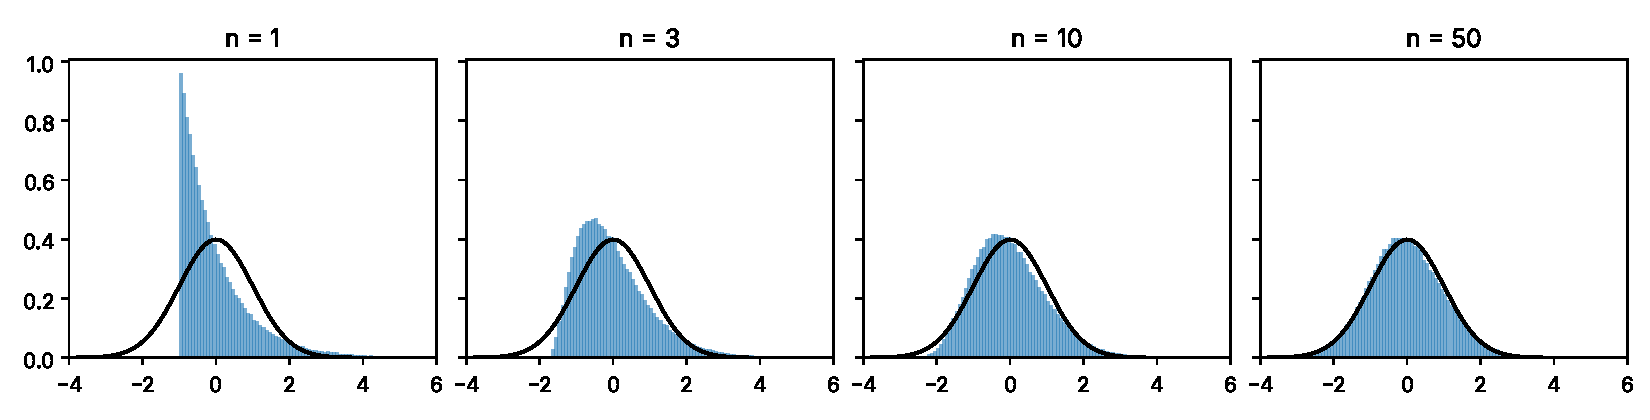
\includegraphics[width=\textwidth]{figures/clt_ustel.pdf}
\caption{Standardised histograms of the sample mean of $\text{Exp}(1)$ variables and the $\Normal(0,1)$ density. The right skewness disappears as $n$ grows.}
\end{figure}

\section{Comments and Notes}

\begin{remark}[What the CLT Does Not Say]
The CLT\index{central limit theorem clt@central limit theorem (CLT)} says that the \emph{distribution} of $Z_n$ converges to the normal; it does not say that $Z_n$ itself converges anywhere (in fact $Z_n$ does not converge in probability\index{convergence in probability@convergence in probability}). Moreover, the convergence is pointwise: for tail probabilities (such as $\P(Z_n>5)$) the relative error may be large; such questions are the subject of large deviations theory.
\end{remark}

\begin{remark}[How Critical the Assumptions Are]
If the finite-variance condition is dropped, the limit may be a \emph{stable} distribution instead of the normal (the Cauchy is a special case), and the scaling becomes $n^{1/\alpha}$ instead of $\sqrt n$. If independence is dropped --- for example in time series --- the variance $\sigma^2$ must be replaced by the long-run variance $\sum_{h}\gamma(h)$.
\end{remark}

\begin{remark}[Link with Chapter~\ref{ch:mle-asimptotik}]
The asymptotic normality\index{asymptotic normality@asymptotic normality} of the MLE comes from the fact that the score is an i.i.d.\ sum to which the CLT applies; the Slutsky\index{slutsky s theorem@Slutsky's theorem} and continuous mapping theorems\index{continuous mapping theorem@continuous mapping theorem} justify replacing the Hessian by a consistent estimate.
\end{remark}

% --- CHAPTER SUMMARY ---
\section{Chapter Summary}
\begin{summary}
\begin{itemize}
  \item Convergence in distribution is convergence of the CDFs at their continuity points (Definition~\ref{def:dagilimda}). It is equivalent to convergence of the expectations of bounded continuous functions (Lemma~\ref{lem:portmanteau}).
  \item The characteristic function is defined for every distribution and determines it uniquely (Theorem~\ref{thm:teklik}). Lévy's continuity theorem (Theorem~\ref{thm:levy}) reduces convergence in distribution to pointwise convergence of CFs.
  \item The central limit theorem (Theorem~\ref{thm:clt}) says that i.i.d.\ sums with finite variance converge to the normal. The Lindeberg--Feller version (Theorem~\ref{thm:lindeberg}) drops the identical-distribution assumption. Berry--Esseen (Theorem~\ref{thm:berry-esseen}) bounds the approximation error by $O(n^{-1/2})$.
  \item The Cramér--Wold device reduces multivariate convergence to univariate linear combinations; this yields the multivariate CLT (Theorem~\ref{thm:cok-degiskenli-clt}).
  \item Slutsky's theorem (Theorem~\ref{thm:slutsky}) and the continuous mapping theorem (Theorem~\ref{thm:cmt}) are the two basic tools of asymptotic inference. For example, replacing $\sigma$ by $S$ does not change the asymptotic distribution.
\end{itemize}
\end{summary}
% --- END OF CHAPTER SUMMARY ---

\paragraph{Further reading.} \cite[Chapter~3]{durrett}, \cite[Sections~25--27]{billingsley}; from a statistical point of view, \cite[Chapters~2--3]{vdv} and \cite{ferguson}.

\section{Exercises}

\begin{exercise}\label{exr:06-1}
Show that for $X\sim\text{Gamma}(\alpha,\beta)$ (rate parametrisation) $\varphi_X(t)=(1-it/\beta)^{-\alpha}$. Use this to find the distribution of a sum of independent Gamma variables (with the same $\beta$).
\hfill\hyperref[coz:06-1]{\footnotesize$\rightarrow$\,Solution}
\end{exercise}

\begin{exercise}\label{exr:06-2}
Show using CFs that if $X_n\sim\text{Bin}(n,\lambda/n)$, then $X_n\dto\text{Poisson}(\lambda)$.
\hfill\hyperref[coz:06-2]{\footnotesize$\rightarrow$\,Solution}
\end{exercise}

\begin{exercise}\label{exr:06-3}
Let the $X_i$ be i.i.d.\ $\text{Uniform}(0,1)$ and $Y_n=n(1-X_{(n)})$. Show via the CDF that $Y_n\dto\text{Exp}(1)$. This result shows that the CLT does not apply to \emph{extreme-value} statistics and that a different scaling ($n$ instead of $\sqrt n$) is needed; relate it to the German tank problem in Chapter~\ref{ch:tamlik}.
\hfill\hyperref[coz:06-3]{\footnotesize$\rightarrow$\,Solution}
\end{exercise}

\begin{exercise}\label{exr:06-4}
Show by a counterexample that $X_n\dto X$ and $Y_n\dto Y$ do \emph{not} imply $X_n+Y_n\dto X+Y$. (Hint: $Y_n=-X_n$.) Discuss why the limit of $Y_n$ in Slutsky's theorem must be a constant.
\hfill\hyperref[coz:06-4]{\footnotesize$\rightarrow$\,Solution}
\end{exercise}

\end{document}
